\documentclass[border=10pt]{standalone}
\usepackage{pgfplots}
\pgfplotsset{compat=newest}

\begin{document}
		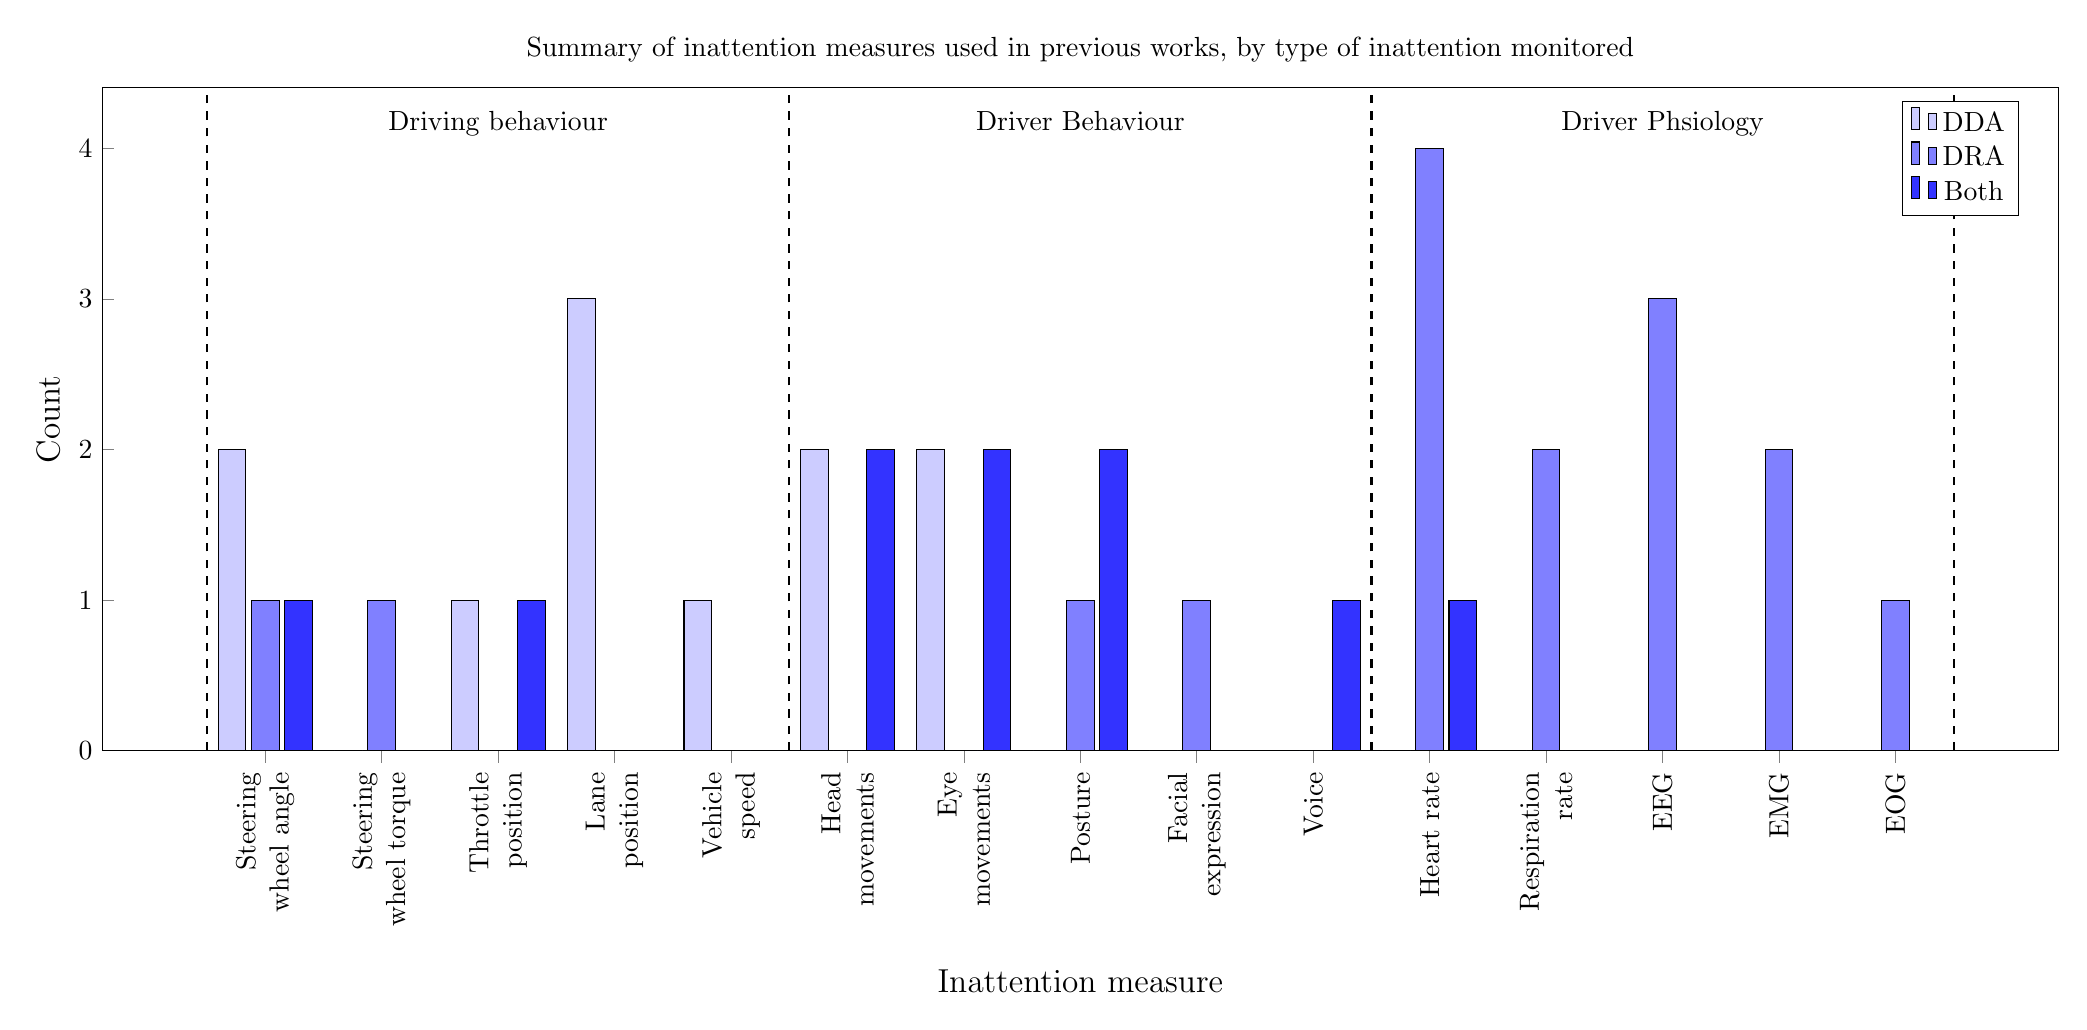
\begin{tikzpicture}
			\begin{axis}[
				title={Summary of inattention measures used in previous works, by type of inattention monitored},
				width=0.95\linewidth,
				ybar,
				ymin=0,
%				axis y line=middle,
%				enlargelimits=0.15,
				xlabel={Inattention measure},
				xlabel style={font=\large},
				ylabel={Count},
				ylabel style={font=\large},				
				xtick=data,
				ytick={0,1,2,3,4},
				xtick pos=left,
				ytick pos=left,
				% use explicit ticklabels instead of symbolc x coords
				xticklabels={%
					Steering\\wheel angle,
					Steering\\wheel torque,
					Throttle\\position,
					Lane\\position,
					Vehicle\\speed,
					Head\\movements,
					Eye\\movements,
					Posture,
					Facial\\expression,
					Voice,
					Heart rate,
					Respiration\\rate,
					EEG,
					EMG,
					EOG},
				xticklabel style={
%					  text width=0.1cm,
%					yshift=-18pt, % move xticks down a bit
					  align=right,
					  rotate=90
				},
				xlabel style={font=\large},
				% extra ticks
				extra x ticks={3,8,13},
				extra x tick labels={Driving behaviour,Driver Behaviour,Driver Phsiology},
				extra x tick style={
					% because the xticklabel style also affects the extra ticks, 
					% shift extra ticklabels back up
					ticklabel style={yshift=8.4cm, rotate=-90,align=center,
					}
					% tickwidth is actually the length of of the ticks (the small lines)
%					tickwidth=0
				},
%				bar width = 5pt,
				x post scale=2.5,
				height=10cm
				]
				%dda
				\addplot+[draw=black,fill=blue!20]
				coordinates{
					(1,2)
					(2,0)
					(3,1)
					(4,3)
					(5,1)
					(6,2)
					(7,2)
					(8,0)
					(9,0)
					(10,0)
					(11,0)
					(12,0)
					(13,0)
					(14,0)
					(15,0)
				};
				%dra
				\addplot+[draw=black,fill=blue!50]
				coordinates{
					(1,1)
					(2,1)
					(3,0)
					(4,0)
					(5,0)
					(6,0)
					(7,0)
					(8,1)
					(9,1)
					(10,0)
					(11,4)
					(12,2)
					(13,3)
					(14,2)
					(15,1)
				};
				%combined
				\addplot+[draw=black,fill=blue!80]
				coordinates{
					(1,1)
					(2,0)
					(3,1)
					(4,0)
					(5,0)
					(6,2)
					(7,2)
					(8,2)
					(9,0)
					(10,1)
					(11,1)
					(12,0)
					(13,0)
					(14,0)
					(15,0)
				};

			\path
			(axis cs:0, \pgfkeysvalueof{/pgfplots/ymin})
			-- coordinate (tmpmin)
			(axis cs:1, \pgfkeysvalueof{/pgfplots/ymin})
			(axis cs:0, \pgfkeysvalueof{/pgfplots/ymax})
			-- coordinate (tmpmax)
			(axis cs:1, \pgfkeysvalueof{/pgfplots/ymax})
			;
			\draw[thick, dashed] (tmpmin) -- (tmpmax);
%
			\path
			(axis cs:5, \pgfkeysvalueof{/pgfplots/ymin})
			-- coordinate (tmpmin)
			(axis cs:6, \pgfkeysvalueof{/pgfplots/ymin})
			(axis cs:5, \pgfkeysvalueof{/pgfplots/ymax})
			-- coordinate (tmpmax)
			(axis cs:6, \pgfkeysvalueof{/pgfplots/ymax})
			;
			\draw[thick, dashed] (tmpmin) -- (tmpmax);
%	
			\path
			(axis cs:10, \pgfkeysvalueof{/pgfplots/ymin})
			-- coordinate (tmpmin)
			(axis cs:11, \pgfkeysvalueof{/pgfplots/ymin})
			(axis cs:10, \pgfkeysvalueof{/pgfplots/ymax})
			-- coordinate (tmpmax)
			(axis cs:11, \pgfkeysvalueof{/pgfplots/ymax})
			;
			\draw[thick, dashed] (tmpmin) -- (tmpmax);
%			
			\path
			(axis cs:15, \pgfkeysvalueof{/pgfplots/ymin})
			-- coordinate (tmpmin)
			(axis cs:16, \pgfkeysvalueof{/pgfplots/ymin})
			(axis cs:15, \pgfkeysvalueof{/pgfplots/ymax})
			-- coordinate (tmpmax)
			(axis cs:16, \pgfkeysvalueof{/pgfplots/ymax})
			;
			\draw[thick, dashed] (tmpmin) -- (tmpmax);
%			
			\legend{DDA,DRA,Both}
			\end{axis}
		\end{tikzpicture}
%
\end{document}